\chapter{Test Appendix with a very long title in order to test spacing behavior} \label{app:test}
\lipsum[2]

A convenient form for representing substantial numerical or textual data is a table. 
Table~\ref{tab:test} shows an example of this functionality in \LaTeX.
\begin{table}
  \centering
  \caption{Test table. With an extra-long caption to test spacing functionality for table captions. And inline mathematics.}
  \begin{tabular}{lrr}
    \toprule
    Heading 1 ($u_x$)  & Head 2 & Head 3 \\
    \midrule
    Analytical         & 1.000  & 1.000  \\
    Forward Difference & 0.973  & 0.976  \\
    \bottomrule
  \end{tabular}
  \label{tab:test}
\end{table}
Diagrams, plots, and other graphics should be placed in figures. 
Figure~\ref{fig:test} shows an example of such an environment.
The command \verb+\includegraphics+ from the \verb+graphicx+ package may be used to include external graphics in a wide variety of formats.
\begin{figure}
  \centering 
  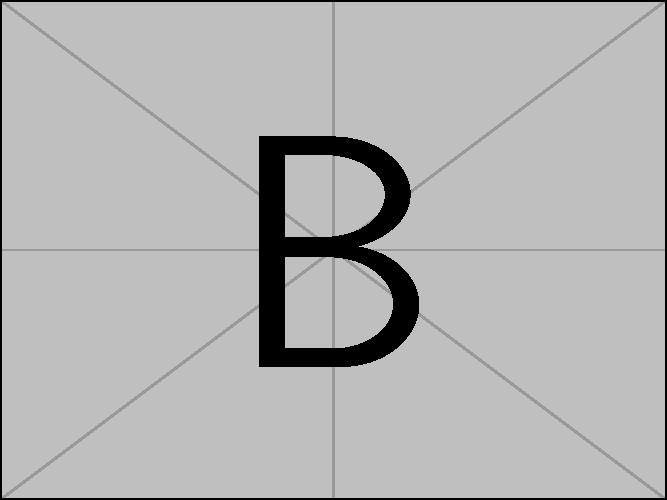
\includegraphics[width=1in]{example-image-b}
  \caption{This test figure tests captions and Table of Contents 
    behavior for lengthy captions.}
  \label{fig:test}
\end{figure}

\section{This is a Very Long Heading to Test the Table of Contents Behavior for Very Long Section Headings}
Sample text. Sample text.

\subsection{This is an Extremely Long Subsection Heading to Test Spacing Behavior for Subsections}
\lipsum[3]

\subsubsection{This is an Extremely Long Subsubsection Heading to Test Spacing Behavior for Subsubsections}
\lipsum[4-5]
